\documentclass[a4paper]{article}

\usepackage{INTERSPEECH2018}
\usepackage{booktabs}
\usepackage{adjustbox}
\usepackage{multirow}
\usepackage{textcomp}

\title{Multilingual Multi-Task Learning for Low-Resource Acoustic Modeling}

\name{Josh Meyer$^1$}
%The maximum number of authors in the author list is twenty. If the number of contributing authors is more than twenty, they should be listed in a footnote or in acknowledgement section, as appropriate.
\address{
  $^1$University of Arizona}
\email{joshua.richard.meyer@gmail.com}

\begin{document}

\maketitle
% 
\begin{abstract}
  
\end{abstract}
\noindent\textbf{Index Terms}: speech recognition, multi-task learning, acoustic modeling





\section{Introduction}

Previous work has shown that performance for a low-resource language on speech recognition can be improved by adding training data from another, resource-rich language. Typically, data from another language is added as a separate task in the Multi-Task Learning framework  \cite{caruana1997} via an additional output layer. The targets for this addititional language have typically been states of context-dependent triphones, defined by some tree clustering algorithm.

This current research builds off the intuition that triphones encode information which is too fine-grained to be maximally useful for language-transfer. Using a higher-level of linguistic abstraction (eg. the monophone), we are able to better extract the kind of language-general information useful in training an acoustic model for some target language.

The intuition being that when adding a source language as an auxialilary task, it would be better to focus on source-language distinctions which are robust and will transfer well to a new, target language.

Each auxiliary task is created by redefining the parameters of the HMM-GMM system used to bootstrap the DNN-hybrid system, such that the phonetic decision tree is cut short.

The target language is Kyrgyz, and the source language is English. Both data come from audiobooks, English being from LibriSpeech and Kyrgyz from the Bizdin.kg project.




\section{Background}


The earliest examples of MTL with multiple languages can be found in \cite{huang2013} and \cite{heigold2013}, who both used triphones from each language as additional tasks. They were interested in improving performance on all languages, not just one target language. These two studies were then followed up in multiple other threads of research. More recently, \cite{grezl2016} found that adding more triphones from a single, well-resourced language (English) actually leads to better performance, but this could be conflated with the fact that they did not use any weighting scheme, and as such, the source language with fewer states and more data would more quickly overfit, leaving less of a chance for the target language to exert influence during backprop.


In another direction, multiple works have investigated MTL for a single language, without any source language transfer. These approaches aim to find tasks which are phonetically relevant to the main task. Both \cite{seltzer2013} and later \cite{huang2015} looked at a very similar approach to what I explore here, with MTL on broader, more abstract phonetic categories for English. They both found improvement on TIMIT, but they didn't investigate multi-lingual transfer. With regards to low-resource languages, \cite{chen2014} and later \cite{chen2015} similarly looked at MTL for a single target language, using graphemes or a universal phoneset as extra targets.



\section{DNN-Hybrid Training as Model Transfer}

The standard DNN-Hybrid approach requires the GMM-HMM system to provide the labels for supervised training. This reliance of the DNN on GMM alignments is actually a form of model transfer, where the DNN is trained to perform the extact same classification as its GMM predecessor. The DNN not only learns the frame alignments from the individual GMMs, but also the DNN indirectly learns the structure of the phonetic decision tree used to define the tied-state system. This is because the output layer of the DNN is trained to predict targets which were defined via leaves of the decision tree.


\begin{figure}[!htb]
  \centering
\minipage{0.5\textwidth}
  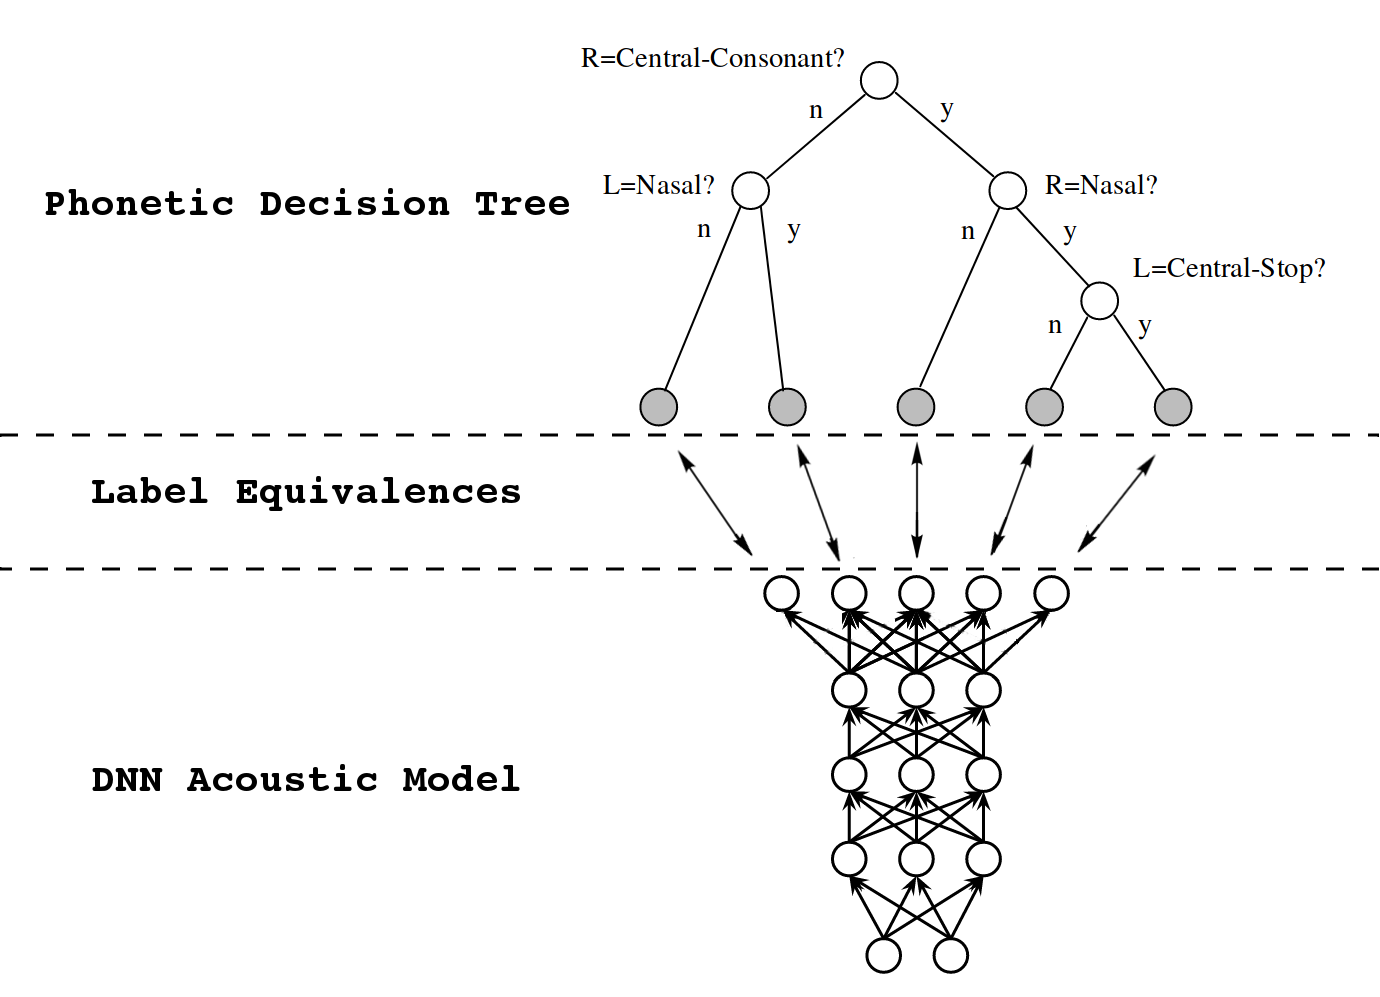
\includegraphics[width=\linewidth]{figs/tree-net.png}
  \caption{GMM$\rightarrow$DNN Model Transfer}
\endminipage\hfill
\end{figure}


Given that standard triphones encode very fine-grained information which may not help performance on a target language, the following experiments investigate GMM$\rightarrow$DNN model transfer at a higher level for an additional source language. 


\section{Experiments}

This work investigates the application of MTL technique to low resource acoustic modeling. All experiments simulate a common development scenario: there exists little transcribed data for the target language, but lots of data in some source language.

The following experiments tease out (1) the level of detail at which the source language should be modeled and (2) the amount of weighting which should be given to the target language training examples.

The first point of interest is the level of detail at which the source language is modeled. This is investigated via addition of multiple tasks to the TDNN during training. The experiements here are crafted to answer the question: \textit{how much phonetic detail should the source language be modeled at to best transfer data to the target language?}.

We can model the source language with lots of contextual detail (ie. the triphone), with abstracted, context-independent detail (ie. the monophone), or somewhere in between. Building of the traditional hybrid DNN-HMM ASR training pipeline, investigating these levels of representation are easily acheived via the phonetic decision tree. We can merely assign labels to training data frames by moving up the tree, from leaves (triphones) to roots (monophones).

The second point of interest is the relative weighting of target vs. source language training data. It is clear that if we train two languages in parallel, the source language (with many more training samples) will dominate the target language in the fight for influence during backprop.

To my knowledge this has not been investigated in ASR acoustic modeling, although it was dedicated its own chapter in Caruana's 1997 dissertation. To investigate weighting further, I examine the following target vs. source weighting schemes: 1-to-2, 1-to-1, and 2-to-1 (all ratios are target-to-source).

These weights are instantiated during training via a weight to the target output label, where the label is a one-hot vector. For example, given 1000 hours of source language and 1 hour of target language, to acheive a 1-to-1 ratio in training, I would multiply the target labels from the target language by 1000, resulting in target vectors such as \texttt{$[0, 0, 0, 0, 1000, 0, 0, \ldots]$} instead of \texttt{$[0, 0, 0, 0, 1, 0, 0, \ldots]$}. The final layer is a ReLU activation, so having a target value higher than $1$ is not an issue as it would be with a traditional softmax layer.



\subsection{Data}

Two speech corpora are used in the following experiments:

\begin{enumerate}
\item $\approx$ 5 hours of LibriSpeech (4.86 hours)
\item $\approx$ 1.5 hours of Kyrgyz audiobook (1.59 hours)
\end{enumerate}

\subsection{Model Building}

All models were build using the Kaldi \texttt{nnet3} approach. The main neural net run script used in this paper can be found at www.github.com/JRMeyer/kaldi-mirror/egs/kgz/kyrgyz-model/run\_nnet3\_multilingual.sh. The main GMM script used to create data alignments can be found at www.github.com/JRMeyer/kaldi-mirror/egs/kgz/kyrgyz-model/run\_gmm.sh.

\subsubsection{Decision Trees}

In GMM training, monophones (for each language) were allotted 1,000 Gaussian components, and trained over 25 iterations of EM. These monophones were then expanded into context-dependent triphones via a phonetic decision tree, with a maximum of 2,000 leaves \& 5,000 Gaussians (LibriSpeech reached 1584 leaves, and Kyrgyz reached 752). The resulting tied-state clusters (ie. leaves) are then trained as context-dedendent triphones over 25 iterations of EM.


\subsubsection{Multi-Task Neural Net Acoustic Models}

Given the alignments from the GMM-HMM models, a 5-layer, 500-dimensional TDNN is trained over 10 epochs of backprop on a single GPU instance.

Each auxiliary task is implemented as a separate output layer along with a separate, penultimate hidden layer. All other hidden layers of the TDNN are trained in parallel.

During testing, \textit{only} the main task is used. The additional tasks are dropped and the baseline Kyrgyz triphones are used in decoding. This highlights the purpose of the extra tasks: to force the learning of robust representations in the hidden layers during training. The tasks may in fact not be the best option for final classification; they serve as ``training wheels'' which are then removed once the net is ready.



\textbf{Baseline Model}

All the following architectures will be compared to the performance of a baseline model of identical architecture (5 hidden layers, 500-dimentional layers, ReLU activations, same training algorithm). The output targets are standard context-dependent triphones trained on Kyrgyz audio.

To account for any advantage mutliple output layers may bring about, the baseline contains two output layers, where the tasks are identical. In this way, random initializations in the weights and biases for each task are accounted for.

\textbf{Auxiliary Tasks}

The auxiliary tasks all train on English language data from the LibriSpeech corpus. Investigating the intuition that labels generated by a standard triphone phonetic decision tree are not the best representation of data for transfer learning, the auxiliary tasks here investigate different levels in the decision tree's branches.

I split the LibriSpeech phonetic decision tree into three logical parts:

\begin{enumerate}
\item roots (standard monophones)
\item branches (what I dub, ``half''-phones)
\item leaves (standard triphones)
\end{enumerate}




\begin{figure}[!htbp]
  \centering
\minipage{0.525\textwidth}
  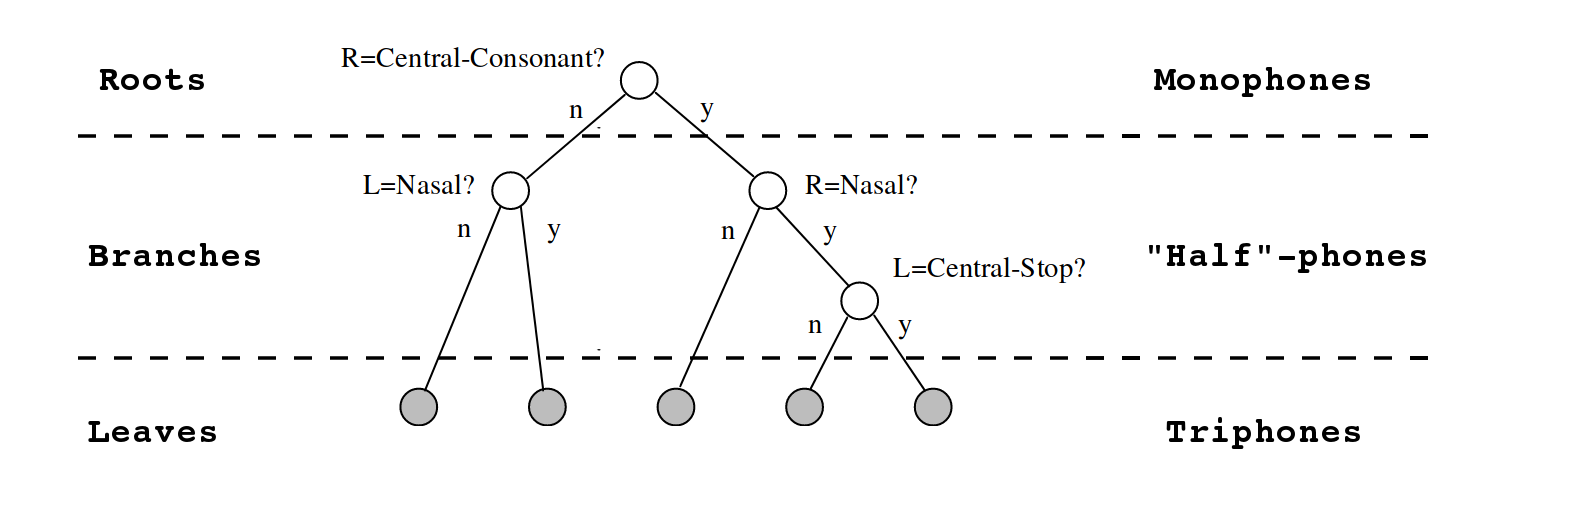
\includegraphics[width=\linewidth]{figs/levels.png}
  \caption{Logical Tree Parts}
\endminipage\hfill
\end{figure}


The ``half''-phones were created by halving the optimal number of leaves from the triphone system (ie. 1584 leaves) and re-training a new GMM-HMM system with half the optimal number of leaves (1/2 * 1584 = 792 leaves). All the other parameters were left unchanged (number of Gaussian components, iterations of EM, etc.). 




\begin{table}[!htbp]
  \centering
    \caption{Auxiliary Tasks}
  \begin{adjustbox}{width=.45\textwidth}
    \begin{tabular}{lcc}
      \toprule
      \textbf{Logical Tree Part} & \textbf{Level of Phonetic Detail} & \textbf{ \textnumero~of Tasks}\\
      \midrule
      Roots & Monophones & 1\\
      Branches & Half-phones & 1\\
      Leaves & Triphones & 1\\ 
      Lower Tree & Monophones + Half-phones & 2\\
      Upper Tree & Half-phones + Triphones & 2\\
      Whole Tree & Monophones + Half-phones + Triphones & 3\\
      \bottomrule
    \end{tabular}
    \label{table:data}
  \end{adjustbox}
\end{table}

Each of the above tasks were trained on the 5 hour section of LibriSpeech corpus. They are included as an extra output layer in the TDNN.


By forcing the neural net to recognize higher levels in the tree, we will learn representations which are more abstract, and therefore more likely to be relevant multi-lingually. 


The addition of each above task adds approximately 5 hours of training data to the standard training of a Single Task Model on Kyrgyz. As such, a weighting procedure was used to balance the relative influence of source vs. target training data on backprop. For example, to reach a one-to-one ratio, where one hour of Kyrgyz is equal to one hour of English, I multiplied every Kyrgyz target one-hot vector by $3.06$.

\begin{table}[!htbp]
  \centering
    \caption{Target:Source Data Weighting Scheme}
  \begin{adjustbox}{width=.3\textwidth}
    \begin{tabular}{cc}
      \toprule
      \textbf{Target:Source Ratio} & \textbf{Target Weight}\\
      \midrule
      1:2 & 1.53x  \\
      1:1 & 3.06x  \\
      2:1 & 6.12x  \\
      \bottomrule
    \end{tabular}
    \label{table:data}
  \end{adjustbox}
\end{table}




\subsection{Results}


All results are performed on the same held-out section of Kyrgyz audiobook. The bigram language model, lexicon, and main-task decision tree are built into a standard decoding graph in the traditional Kaldi style. Decoding is performed with a bigram backoff language model trained on a Wikipedia Kyrgyz dump, and contains, 103,998 unigrams and 56,6871 bigrams.


\begin{enumerate}
\item Any amount of English beats out Kyrgyz-only baseline.
\item Triphones work better than monophones (except for the 2-to-1 weighting).
\item Both languages / tasks overfit (referencing frame-classification logs)
\item atai overfit slower with additional tasks
\item atai overfits with monophones earlier, I think because it's an easier task
\item only train on 30 minutes of Krygyz... more likely to find an effect
\end{enumerate}




\begin{table}[!htbp]
  \centering
    \caption{TDNN // 5-layer // 500-dim //  10 epoch }
  \begin{adjustbox}{width=.45\textwidth}
    \begin{tabular}{lccc}
      \toprule
      & \multicolumn{3}{c}{\textbf{Target:Source Weighting}} \\
      \textbf{Auxiliary (Source Lang) Tasks} & \textit{1-to-2} & \textit{1-to-1} & \textit{2-to-1}\\
      \midrule
      STL Baseline                          &  \multicolumn{3}{c}{50.54}  \\
      Monophones                            &  3.13  & 3.22 & 2.34  \\
      Halfphones                            &  1.86  & \textbf{3.81} & 1.86 \\
      Triphones                             &  \textbf{3.81} & 3.42 & 1.17  \\
      Monophones + Halfphones               &  2.44  & 2.05 &  2.34\\
      Halfphones + Triphones                &  2.64  & 2.54 & \\
      Monophones + Halfphones + Halfphones  &  1.95  & 2.34 & \\
      \midrule
      AVERAGE                               &  2.64  & 2.90 & \\
      \bottomrule
    \end{tabular}
    \label{table:data}
  \end{adjustbox}
\end{table}


%% \begin{table}[!htbp]
%%   \centering
%%     \caption{TDNN // 5-layer // 500-dim //  10 epoch }
%%   \begin{adjustbox}{width=.45\textwidth}
%%     \begin{tabular}{lccc}
%%       \toprule
%%       & \multicolumn{3}{c}{\textbf{Target:Source Weighting}} \\
%%       \textbf{Auxiliary (Source Lang) Tasks} & \textit{1-to-2} & \textit{1-to-1} & \textit{2-to-1}\\
%%       \midrule
%%       STL Baseline                          &  \multicolumn{3}{c}{50.54}  \\
%%       Monophones                            &  47.41  & 47.32 & 48.20  \\
%%       Halfphones                            &  48.68  & 46.73 & 48.68 \\
%%       Triphones                             &  46.73  & 47.12 & 49.37  \\
%%       Monophones + Halfphones               &  48.10  & 48.49 & 48.20 \\
%%       Halfphones + Triphones                &  47.90  & 48.00 & \\
%%       Monophones + Halfphones + Halfphones  &  48.59  & 48.20 & \\
%%       \bottomrule
%%     \end{tabular}
%%     \label{table:data}
%%   \end{adjustbox}
%% \end{table}





\section{Discussion}


\section{Conclusions}

\section{Acknowledgements}


\newpage

\bibliographystyle{IEEEtran}
\bibliography{mybib}



\end{document}
